\documentclass{article}

\usepackage[utf8x]{inputenc} 
\usepackage[T1]{fontenc}      
\usepackage[francais]{babel} 
\usepackage[top=3cm, bottom=3cm, left=3cm, right=3cm]{geometry}
\usepackage{graphicx}
\graphicspath{{../sources/images/diagrammesUML/}}
\usepackage{wrapfig}

\title{Conception bibliothèques graphes rotor}
\author{Clément \bsc{Chrétien} \and Thomas \bsc{Petiteau}}

\begin{document}
	\maketitle
	\clearpage
	
	\tableofcontents
	\clearpage

	\section{Introduction}
		\paragraph*{}
		Le présent document a pour but d'expliquer la conception faite d'une bibliothèque pour la manipulation de graphes rotors, développée pour le logiciel Sagemath. L'objectif est ici de détailler l'ensemble des choix pris au cours du développement et l'origine de ces mêmes choix.
	
	\section{Place dans sagemath}
		\paragraph*{}
		L'ensemble de la bibliothèque développée a été regroupé dans un \textit{package} nommé "rotor". Il n'est cependant pas exclu d'intégrer la bibliothèque au \textit{package} "graph" qui regroupe l'ensemble des classes et outils permettant d'appliquer la théorie des graphes et ceux, en fonction de la taille finale du \textit{package} "rotor".
	
	\section{Classes}
		\paragraph*{}
		La figure \ref{fig:diagClassGlobal} montre l'ensemble des classes composant le \textit{package} rotor ainsi que l'association entre ce dernier et le \textit{package} "graphe", déjà présent sur sagemath.
		
		\begin{figure}[h]
			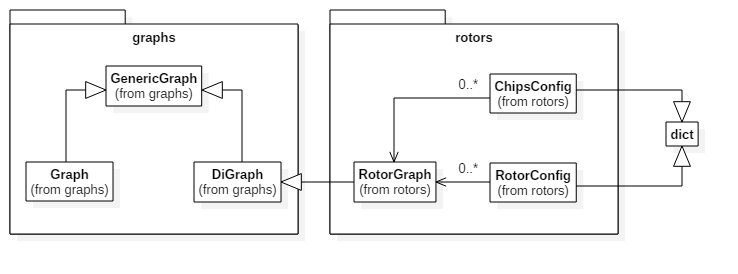
\includegraphics[width=10cm]{diagClassGlobal.png}
			\centering
			\caption{Diagramme de classe UML montrant le \textit{package} "rotor" et son attachement au \textit{package} "graphe"}
			\label{fig:diagClassGlobal}
		\end{figure}
	
		\subsection{RotorGraph}
			\label{sec:RotorGraph}
			\paragraph*{}
			La classe "RotorGraph" représente un graphe orienté (elle hérite de la classe "DiGraph") sur laquelle on apporte les informations nécessaires à un graphe rotor. La figure \ref{fig:diagClassRotorGraph} montre l'ensemble des champs et méthodes de la classe "RotorGraph" à l'aide d'un diagramme de classe UML.
			
			\begin{figure}[h]
				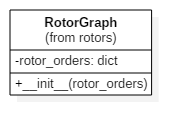
\includegraphics[width=4cm]{diagClassRotorGraph.png}
				\centering
				\caption{Diagramme de classe UML montrant la classe "RotorGraph"}
				\label{fig:diagClassRotorGraph}
			\end{figure}
			
			\subsubsection{Champs}
				\label{sec:RotorGraph-Champ}
				\begin{itemize}	
					\item \textbf{rotor\_orders}\newline
					Il s'agit d'un dictionnaire associant à chaque sommet du graphe une liste composé de ses voisins (chaque voisin pouvant apparaître 0 ou plusieurs fois). Par défaut, la liste de "rotor\_order" d'un sommet sera égale à la liste de ses voisins sortants.
				\end{itemize}
		
			\subsubsection{Méthodes}
				\begin{itemize}
					\item \textbf{\_\_init\_\_}\newline
					Le constructeur de la classe. Héritant de la classe "DiGraph", ce constructeur prend en entrée les même paramètres qui ont été omis sur la figure \ref{fig:diagClassRotorGraph} pour en faciliter la lecture. Le paramètre rajouté à ce constructeur est "rotor\_orders".
					\begin{itemize}
						\item \textit{rotor\_orders}\newline
						Dictionnaire associant à un sommet une liste donnant l'ordre de rotation du rotor (voir le champ "rotor\_orders" de la classe "RotorGraph", voir \ref{sec:RotorGraph-Champ}). Tout sommet ne figurant pas dans le dictionnaire sera initialisé comme étant égal à la liste de ses voisins sortants. 
					\end{itemize}
					\item \textbf{default\_config}\newline
					Renvoie la configuration de rotor par défaut du graphe appelant (Tous les rotors pointent vers le premier voisins de leur liste d'ordre de rotor)
				\end{itemize}
	
		\subsection{RotorConfig}
			\paragraph*{}
			La classe "RotorConfig" représente une configuration de rotors pour un graphe rotor (objet de la classe "RotorGraph", voir \ref{sec:RotorGraph}). La figure \ref{fig:diagClassRotorConfig} montre l'ensemble des champs et méthodes de la classe "RotorConfig" à l'aide d'un diagramme de classe UML.
			
			\begin{figure}[h]
				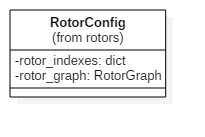
\includegraphics[width=5cm]{diagClassRotorConfig.png}
				\centering
				\caption{Diagramme de classe UML montrant la classe "RotorConfig"}
				\label{fig:diagClassRotorConfig}
			\end{figure}
			
			\subsubsection{Champs}
				\begin{itemize}	
					\item \textbf{rotor\_indexes}\newline
					Il s'agit d'un dictionnaire associant à chaque sommet, l'indice dans sa liste de "rotor\_orders" (voir \ref{sec:RotorGraph-Champ}) du voisin vers lequel le rotor est dirigé.
					\item \textbf{rotor\_graph}\newline
					Le graphe rotor (classe "RotorGraph", voir \ref{sec:RotorGraph}) auquel est associé la configuration de rotor.
				\end{itemize}
            
            \subsubsection{Méthodes}
                \begin{itemize}
                    \item \textbf{\_\_init\_\_}\newline
                    Constructeur de la classe.
                    \begin{itemize}
                        \item \textit{rotor\_graphe}\newline
                        le graphe rotor (objet de la classe "RotorGraph", voir \ref{sec:RotorGraph}) auquel la configuration de \textit{rotor} est associée.
                        \item \textit{rotor\_indexes}\newline
                        L'index du rotor associé à chaque sommets. Le paramètre peut être de plusieurs types :
                        \begin{itemize}
                            \item dict : un dictionnaire associant à chaque sommet l'index du sommet vers lequel le \textit{rotor} pointe. Les sommets non donnés sont initialisé à zéro \textit{chips}
                            \item list : chaque élément de la liste étant l'index du sommet vers lequel le rotor pointe. Si la liste est plus petite, elle est complétée par des zéro.
                            \item autres types : tous les index sont mis à zéro.
                        \end{itemize}
                    \end{itemize}
                    \item \textbf{indexes}\newline
                    Permet de récupérer ou de modifier le paramètre \textit{rotor\_indexes}.
                    \item \textbf{rotor}\newline
                    Permet de récupérer ou de modifier le paramètre \textit{rotor\_graphe}.
                    \item \textbf{pointed\_vertex}\newline
                    Permet de récupérer l'indice du sommet sur lequel le rotor du sommet donné en paramètre pointe.
                    \item \textbf{pointed\_vertices}\newline
                    Permet de récupérer l'indice de tous les sommets sur lesquels le rotor des sommets du graphe donné en paramètre pointe grâce au dictionnaire donné en paramètre.
                    \item \textbf{change\_rotor\_position}\newline
                    Permet de changer l'indice du sommet sur lequel le rotor du sommet donné en paramètre pointe.
                    \item \textbf{change\_rotors\_positions}\newline
                    Permet de changer l'indice de tous les sommets sur lesquels le rotor des sommets du graphe donné en paramètre pointe grâce au dictionnaire donné en paramètre.
                \end{itemize}
	
		\subsection{ChipsConfig}
			\paragraph*{}
			La classe "ChipsConfig" représente une configuration de \textit{chips} pour un graphe rotor (objet de la classe "RotorGraph", voir \ref{sec:RotorGraph}). La figure \ref{fig:diagClassChipsConfig} montre l'ensemble des champs et méthodes de la classe "ChipsConfig" à l'aide d'un diagramme de classe UML.
			
			\begin{figure}[h]
				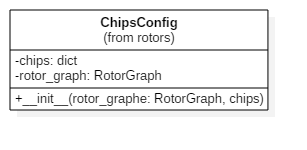
\includegraphics[width=5cm]{diagClassChipsConfig.png}
				\centering
				\caption{Diagramme de classe UML montrant la classe "ChipsConfig"}
				\label{fig:diagClassChipsConfig}
			\end{figure}
		
			\subsubsection{Champs}
				\begin{itemize}
					\item \textbf{chips}\newline
					Il s'agit d'un dictionnaire associant à chaque sommet le nombre de \textit{chips} présent dessus.
					\item \textbf{rotor\_graph}\newline
					Le graphe rotor (classe "RotorGraph", voir \ref{sec:RotorGraph}) auquel est associé la configuration de rotor
				\end{itemize}
		
			\subsubsection{Méthodes} 
				\begin{itemize}
					\item \textbf{\_\_init\_\_}\newline
					Constructeur de la classe.
					\begin{itemize}
						\item \textit{rotor\_graphe}\newline
						le graphe rotor (objet de la classe "RotorGraph", voir \ref{sec:RotorGraph}) auquel la configuration de \textit{chips} est associée.
						\item \textit{chips}\newline
						Les \textit{chips} à placer sur les différents sommets du graphe. Le paramètre peut être de plusieurs types:
						\begin{itemize}
							\item dict : un dictionnaire associant à chaque sommet le nombre de \textit{chips} placées dessus. Les sommets non donnés sont initialisé à zéro \textit{chips}
							\item list : chaque élément de la liste étant le nombre de chips à placer sur le sommet d'indice correspondant dans la liste des sommets du graphe rotor associé. Si la liste est plus petite, elle est complétée par des zéro.
							\item autres types : toutes les chips sont mises à zéro.
						\end{itemize}
					\end{itemize}
					\item \textbf{values}\newline
					Retourne le nombre de \textit{chips} placées sur chaque sommet sous forme de liste ordonnée selon les vecteurs du graphe rotor associé.
					\item \textbf{chips\_count}\newline
					Retourne le nombre de \textit{chips} placée sur un sommet le nombre total de chips si aucun sommet n'est donné
					\begin{itemize}
						\item \textit{vertex}\newline
						le sommet dont on cherche le nombre de \textit{chips}
					\end{itemize}
					\item \textbf{add\_chips\_to\_vertex}\newline
					Ajoute un nombre donné de \textit{chips} sur le sommet donné.
					\begin{itemize}
						\item \textit{quantity}\newline
						Le nombre de chips à ajouter.
						\item \textit{vertex}\newline
						Le sommet sur lequel ajouter les \textit{chips}
					\end{itemize}
					\item \textbf{sub\_chips\_to\_vertex}\newline
					Retire un nombre donné de \textit{chips} sur le sommet donné.
					\begin{itemize}
						\item \textit{quantity}\newline
						Le nombre de chips à retirer.
						\item \textit{vertex}\newline
						Le sommet sur lequel retirer les \textit{chips}.
					\end{itemize}
					\item \textbf{add\_chips\_to\_vertices}\newline
					Ajoute un nombre donné de \textit{chips} sur les sommets donnés.
					\begin{itemize}
						\item \textit{quantity}\newline
						Le nombre de chips à ajouter.
						\item \textit{vertex}\newline
						Les sommets sur lesquels ajouter les \textit{chips}
					\end{itemize}
					\item \textbf{sub\_chips\_to\_vertices}\newline
					Retire un nombre donné de \textit{chips} sur les sommets donnés.
					\begin{itemize}
						\item \textit{quantity}\newline
						Le nombre de chips à retirer.
						\item \textit{vertex}\newline
						Les sommets sur lesquels retirer les \textit{chips}.
					\end{itemize}
					\item \textbf{add\_chips}\newline
					Ajoute les \textit{chips} données à la configuration
					\begin{itemize}
						\item \textit{chips}\newline
						dictionnaire associant à un sommet le nombre de chips à lui ajouter
					\end{itemize}
					\item \textbf{sub\_chips}\newline
					Retire les \textit{chips} données à la configuration
					\begin{itemize}
						\item \textit{chips}\newline
						dictionnaire associant à un sommet le nombre de chips à lui retirer
					\end{itemize}
				\end{itemize}
	
\end{document}
	
	